\documentclass{beamer}
\usepackage[backend=bibtex,style=trad-plain, citestyle=verbose]{biblatex}

% For more themes, color themes and font themes, see:
% http://deic.uab.es/~iblanes/beamer_gallery/index_by_theme.html
%
\mode<presentation>
{
  \usetheme{Darmstadt}       % or try default, Darmstadt, Warsaw, ...
  \usecolortheme{default} % or try albatross, beaver, crane, ...
  \usefonttheme{serif}    % or try default, structurebold, ...
  \setbeamertemplate{navigation symbols}{}
  \setbeamertemplate{}[numbered]
} 
\makeatletter
\setbeamertemplate{footline}
{
  \leavevmode%
  \hbox{%
  \begin{beamercolorbox}[wd=.333333\paperwidth,ht=2.25ex,dp=1ex,center]{author in head/foot}%
    \usebeamerfont{author in head/foot}
  \end{beamercolorbox}%
  \begin{beamercolorbox}[wd=.333333\paperwidth,ht=2.25ex,dp=1ex,center]{title in head/foot}%
    \usebeamerfont{title in head/foot}
  \end{beamercolorbox}%
  \begin{beamercolorbox}[wd=.333333\paperwidth,ht=2.25ex,dp=1ex,right]{date in head/foot}%
    \usebeamerfont{date in head/foot}\insertshortdate{}\hspace*{2em}
    \insertframenumber{} / \inserttotalframenumber\hspace*{2ex} 
  \end{beamercolorbox}}%
  \vskip0pt%
}
\makeatother

\usepackage[english]{babel}
\usepackage[utf8]{inputenc}
\usepackage{chemfig}
\usepackage[version=3]{mhchem}
\usepackage{subfigure}
\usepackage{graphicx}
\usepackage{wasysym}
\usepackage{relsize}
\usepackage{color}

\newcommand{\bigqm}[1][1]{\text{\larger[#1]{\textbf{?}}}}
\newcommand*{\vimage}[2]{\vcenter{\hbox{\includegraphics[#1]{#2}}}}
\newcommand*{\vpointer}{\vcenter{\hbox{\scalebox{2}{\Huge\pointer}}}}
\newcommand\tab[1][1cm]{\hspace*{#1}}

\bibliography{Presentation}
\bibstyle{plain}
\definecolor{mygray}{gray}{0.6}

% On Overleaf, these lines give you sharper preview images.
% You might want to `comment them out before you export, though.
\usepackage{pgfpages}
\pgfpagesuselayout{resize to}[%
  physical paper width=8in, physical paper height=6in]

% Here's where the presentation starts, with the info for the title slide
\title{Chapter 14 -  Experimentation}
\author{Daniel Seidinger\\
Brikena Celaj}
\date{02.11.2018}

\begin{document}

\begin{frame}
  \titlepage
\end{frame}

\begin{frame}{Experiments}
\begin{block}{Zobel 197}
Experiments are an essential part of sound science
\end{block}

\begin{block}{ Zobel 198}
Tests should be fair rather than constructed to support the hypothesis
\end{block}
\end{frame}

\section{Baseline and Data}
\begin{frame}{Baseline}
First steps:
\begin{itemize}
\item Identify an appropriate Baseline
\item Existing methods already good enough?
\item Barrier to entry: Must be familiar with existing methods/ideas 
\end{itemize}
BUT: No excuse for poor science!
\end{frame}

\begin{frame}{Baseline}
\begin{alertblock}{Possible Problems}
\begin{itemize}
\item Baseline is not updated 
\item Widely available implementation is used as a reference point
\item[] $\rightarrow$ Improvements may not be cummulative
\item No clear baseline
\end{itemize}
\end{alertblock}
\end{frame}

\begin{frame}{Persuasive Data}
\begin{itemize}
\item Access and understanding of the appropriate data is critical for experiments
\end{itemize}
\begin{block}{Things to Consider}
\begin{itemize}
\item What data is available, what is the source
\item What specific mechanisms to gather and standardize
\item Will the data be sufficient in volume/quality
\item What domain knowledge is needed to interpret the data
\item Limits, biases, flaws and properties of the data and how this is managed
\item What will the results be if the data supports/opposes the hypothesis 
\end{itemize}
\end{block}
\end{frame}


\begin{frame}{Persuasive Data}
\begin{block}{Do's and Don'ts}

\begin{itemize}
\item Before committing to a research question, be sure that you are able to obtain the needed data
\item Have sufficient data sets
\item Test on volumes of data you are making the claims on
\end{itemize}

\end{block}
\end{frame}

\begin{frame}{Persuasive Data}
\begin{block}{Do's and Don'ts}

\begin{itemize}
\item Distinguish between observation phase and confirmation phase
\item Choosing parameters to suite data or vice versa invalidates the research
\item Identify data/input for which the hypothesis is least likely to hold, these are the interesting cases
\end{itemize}

\end{block}
\end{frame}


\section{Interpretation}
\begin{frame}{Interpretation}
The experiment yielded results (hopefully), what now? \\
\begin{itemize}
\item Are there other possible interpretations?
\item[] $\rightarrow$ Further tests to eliminate them
\item Careful with failed experiments

\end{itemize}
\color{red} $\times$ \color{black} "We have shown that it is not possible to
make further improvement" \\
\color{green} \checkmark \color{black} Redesign, likely a problem in the test not hypothesis
\end{frame}

\begin{frame}{Interpretation}
\begin{itemize}
\item  Success in special case $\not =$ Success in general
\item Don't draw undue conclusions or overstate them
\item Ordinal better than interval/ratio
\begin{block}{Zobel 205}
A key concept here is of predictivity. The main reason that we experiment and
measure is to provide evidence about the behaviour of a system in general [...].
\end{block}
\end{itemize}
\end{frame}


\section{Robustness}
\begin{frame}{Robustness}
Properties of robust experiments:
\begin{itemize}

\item Independent of quality of implementation 
\item Yield \color{green}\checkmark \color{black}  or \color{red} $\times$ \color{black} 
\item Demonstrate a trend or pattern
\item Success is obvious, not a subject to interpretation

\end{itemize}
\end{frame}

\begin{frame}{Robustness - Speed Experiments}
\begin{block}{Speed Experiments}
\begin{itemize}
\item Maximum, minimum, average or median time 
\item Care for anomalies and don't just discard them
\item Explain/discuss them
\end{itemize}
$\rightarrow$ More in Chapter 15
\end{block}

\end{frame}

\begin{frame}
\begin{itemize}
\item Compare components, not only as a whole
\item investigate relevant variables separately
\item Measuring distributed algorithms may be difficult 
\end{itemize}
\begin{block}{Zobel 207}
To produce strong experimental designs [...], researchers need to use their understanding [...] of the algorithms to
anticipate whether issues of robustness will arise.
\end{block}

\end{frame}

\section{Performance of Algorithms}
\begin{frame}{Performance of Algorithms}
\onslide<1->{
 \textbf{Tools:}\\
\begin{itemize}
\item Formal proof
\item Mathematical modeling
\item Simulation and
\item Experimentation
\end{itemize} 

}

\onslide<2>{
 \textbf{Constraints:}\\
\begin{itemize}
\item Basis evaluation
\item Processing time
\item Memory and disk requirements
\item Disk and network traffic
\item Applicability
\end{itemize}
}
\end{frame}

\begin{frame}{Performance of Algorithms}

\onslide<1->{
 \textbf{Basis of evaluation}\\
\begin{itemize}
\item Comparison of the algorithm
\item If the basis of comparison is questionable, the results are questionable too
\end{itemize} 

}
\onslide<2-3>{
 \textbf{Processing time}\\
\begin{itemize}
\item Time is one of the principal resources used by algorithm
\item Not always easy to measure
\end{itemize}
}
\onslide<3>{
 \textbf{Memory and disk requirements}\\
\begin{itemize}
\item Specify how your algorithms use memory
\end{itemize}
}
\end{frame}

\begin{frame}{Performance of Algorithms }
\onslide<1->{
\textbf{Disk and network traffic}\\
\begin{itemize}
\item Disk costs have two components, the time to fetch the first bit of requested data  and the time required to transmit the requested data
\item Similar with network traffic
\item Describe disk performance with approximations 
\end{itemize}
}
\onslide<2>{
 \textbf{Applicability}\\
\begin{itemize}
\item Comparison with regard to functionality
\item A common error - comparison of two algorithms that perform different tasks
\end{itemize}
}
\end{frame}



\begin{frame}{Human Studies }
\onslide<1->{
Humans resolve many research questions:
\begin{itemize}
\item \tab Has the compressed image adequate quality? \\
\item \tab Are the responses of the search engine useful?\\
\item \tab Did the robot do a good job?\\
\end{itemize}
}
\onslide<2>{
\vspace{5mm}
Researchers should answer these questions:
\begin{itemize}
\item \tab Are humans subjects need in the research? \\
\item \tab How many humans will be needed?\\
\item \tab What instructions will they be given?\\
\end{itemize}
}
\end{frame}
\begin{frame}{Human Studies }
\onslide<1->{
\begin{itemize}
\item Human studies are an essential element of computer science
\end{itemize}
}

\onslide<2>{
\begin{itemize}
\item  Users have a great impact on many outputs\\
\begin{itemize}
 \item[--] \footnotesize Strong conclusions concerning a user interface\\
 \item[--] \footnotesize Better search mechanisms\\
 \item[--] \footnotesize Strong results on machine translation\\
\end{itemize}
\end{itemize}
}

\end{frame}





\begin{frame}{Coding for Experimentation }
\onslide<1->{
\begin{itemize}
\item The Basic rule\\
\tab \footnotesize Keep things simple!
\end{itemize}
}
\onslide<2-5>{
\begin{itemize}
\item One task, one tool\\
\tab \footnotesize Decompose the problem into separate pieces of code
\end{itemize}
}
\onslide<3-5>{
\begin{itemize}
\item Cut the right corners\\
\tab \footnotesize Code, if you have to run the experiment again
\end{itemize}
}
\onslide<4-5>{
\begin{itemize}
\item Use the right tool, not the most convenient one
\end{itemize}
}
\onslide<5>{
\begin{itemize}
\item Verify the correctness of the output
\end{itemize}
}
\end{frame}

\begin{frame}{Coding for Experimentation}
\onslide<1->{
 \textbf{Using Unix}\\
\begin{itemize}
\item Usually - Run in command-line
\item More reliable - Run all experiments from scripts
\end{itemize} 
}
\onslide<2>{
\vspace{5mm}
 \textbf{Feasibility}
\begin{itemize}
\item Large volumes of data
\item Implementation of production quality code
\item Use humans for evaluation of results
\item Use of particular pieces of software
\end{itemize}
}

\end{frame}

\begin{frame}{Describing Experiments}
\onslide<1->{
\begin{itemize}
\item Analyze the results\\
\tab \footnotesize Explain the results by confirming or disproving the hypothesis
\end{itemize} 
}
\onslide<2>{
\begin{figure}
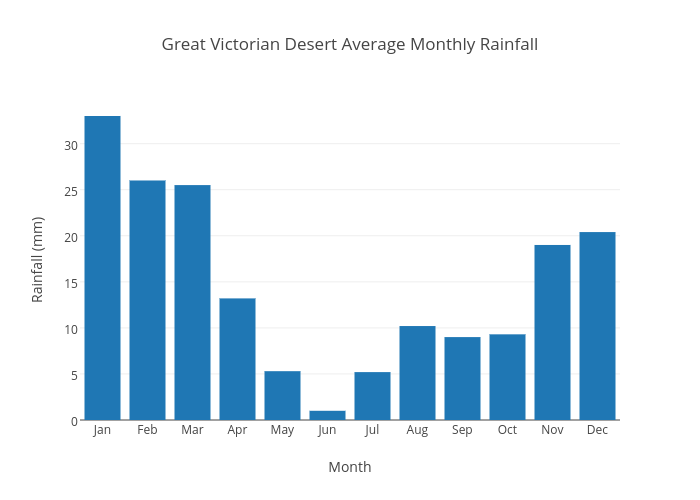
\includegraphics[scale = 0.2]{fig/pic10}
\vspace{10cm}
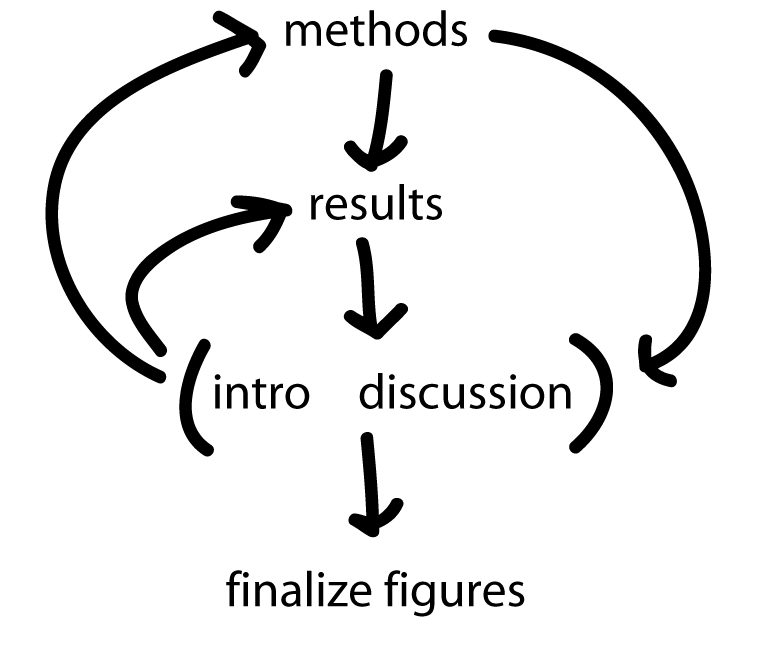
\includegraphics[scale=0.16]{fig/pic12}
\end{figure}
}
\end{frame}

\begin{frame}{Describing Experiments}
\onslide<1->{
\begin{itemize}
\item Decide which results to report\\
\tab \footnotesize Do not show the material with no interest to others
\end{itemize} 
}
\onslide<2-3>{
\begin{itemize}
\item State the existence of failure\\
\tab \footnotesize If a test fails on some data sets and succeeds on others, it is unethical to hide the failures
\end{itemize} 
}
\onslide<3>{
\begin{itemize}
\item Experiment relevance to the hypothesis\\
\tab \footnotesize Some experiments may lead to a dead end
\end{itemize} 
}
\end{frame}

\begin{frame}{Describing Experiments}
\onslide<1->{
\begin{itemize}
\item Describe the data\\
\tab \footnotesize How the data was gathered or created
\end{itemize} 
}

\onslide<2-3>{
\begin{itemize}
\item Notebooks\\
\tab \footnotesize Strategy used by researchers in other departments of science
\end{itemize} 
}
\onslide<3>{
\begin{itemize}
\item Online coding\\
\tab \footnotesize Strategy used in computer science keeps researchers honest
\end{itemize} 
}
\end{frame}

\begin{frame}{Discussion}
\onslide<1->{
\begin{center} Thank you for your attention!\\
 Question?
\end{center}

}
\end{frame}

\end{document}
